As a review, here are examples of the three types of tree traversals along with
pseudocode for printing all of the nodes in the binary tree:\\
\vspace{0.1cm}
\begin{figure}[H]
    \centering
    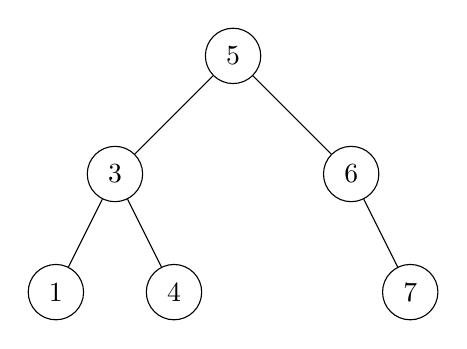
\begin{tikzpicture}[level distance=1.5cm,
        level 1/.style={sibling distance=3cm},
        level 2/.style={sibling distance=1.5cm},
        every node/.style = {minimum width = 2em, draw, circle}
        ]
        \node {5}
            child {node {3}
                child {node {1}}
                child {node {4}}
            }
            child {node {6}
                child {edge from parent[draw = none]}
                child {node {7}}
            };
    \end{tikzpicture}
\end{figure}
\vspace{0.5cm}\\
\begin{minipage}{0.32\textwidth}
\RestyleAlgo{ruled} 
\centering
\begin{algorithm}[H]
    \caption{Inorder}\label{inorder}
    \DontPrintSemicolon
    \SetKwFunction{FInorder}{Inorder}
    \SetKwProg{Fn}{Function}{}{\KwRet}
    \Fn{\FInorder{curr}}{
        \If{curr is null}{
            return\;
        }
        print(node)\;
        Inorder(node.left)\;
        Inorder(node.right)\;
    }
\end{algorithm}
\textbf{Inorder:} 1 3 4 5 6 8
\end{minipage}
\begin{minipage}{0.32\textwidth}
\RestyleAlgo{ruled} 
\centering
\begin{algorithm}[H]
    \caption{Preorder}\label{preorder}
    \DontPrintSemicolon
    \SetKwFunction{FPreorder}{Preorder}
    \SetKwProg{Fn}{Function}{}{\KwRet}
    \Fn{\FPreorder{curr}}{
        \If{curr is null}{
            return\;
        }
        Preorder(node.left)\;
        print(node)\;
        Preorder(node.right)\;
    }
\end{algorithm}
\textbf{Preorder:} 5 3 1 4 6 7
\end{minipage}
\begin{minipage}{0.32\textwidth}
\centering
\RestyleAlgo{ruled} 
\begin{algorithm}[H]
    \caption{Postorder}\label{postorder}
    \DontPrintSemicolon
    \SetKwFunction{FPostorder}{Postorder}
    \SetKwProg{Fn}{Function}{}{\KwRet}
    \Fn{\FPostorder{curr}}{
        \If{curr is null}{
            return\;
        }
        Postorder(node.left)\;
        Postorder(node.right)\;
        print(node)\;
    }
\end{algorithm}
\textbf{Postorder:} 1 4 3 7 6 5
\end{minipage}
\vspace{0.5cm}\\

Printing is relatively straight forward given the ease with which you can
recursively traverse and print nodes from a tree. Your task will be to modify
this approach such that your methods return a list of references to the nodes
in the order of the respective method's traversal. Though this can be done either
iteratively or recursively we will be requiring you to form an iterative solution 
for this set of methods. Consider the details on the differences and similarities
between recursive and iterative traversals of trees at the beginning of the lab
to form this transformation (Section~\ref{sec:traversals}).

\vspace{0.5cm}\\
\textbf{Your Task: } Implement the following methods that use the
aforementioned traversals and return an \lstinline|List| of
references the instances of \lstinline|TreeNode| in the tree.
\begin{enumerate}
    \item \lstinline|public List<TreeNode> getInorderTraversal(){ ... }|
    \item \lstinline|public List<TreeNode> getPostorderTraversal(){ ... }|
    \item \lstinline|public List<TreeNode> getPreorderTraversal(){ ... }|
\end{enumerate}


